\documentclass{article} % For LaTeX2e
\usepackage{final_project,times}
\usepackage{graphicx}
\usepackage{epstopdf}
\usepackage[font=small,labelfont=bf]{caption}
\usepackage[]{algorithm2e}
%\documentstyle[nips12submit_09,times,art10]{article} % For LaTeX 2.09


\title{STA 571 - Deep Neural Network Classifier of Handwritten Digits}


\author{
Mohammed Reza Sanatkar \\
\texttt{reza.sanatkar@duke.edu} \\
\textbf{Mengke Lian} \\
\texttt{mengke.lian@duke.edu}
}

\newcommand{\fix}{\marginpar{FIX}}
\newcommand{\new}{\marginpar{NEW}}

\nipsfinalcopy

\begin{document}


\maketitle

\begin{abstract}
This course project aims at dealing with hand writing recognition task.
Deep neural networks have garnered a lot of attention in the field of machine learning in the recent years.
In this project, we implement a multi-layer neural networks to perform the task of handwritten digits.
Two different methods are employed to train a three layer neural networks. The first used method is the standard back propagation (BP) algorithm. The second method is the combination of the conventional back propagation and restricted Boltzmann machine (RBM).  
For BP, the generalization error is $3.75\%$, while for the second method which is the combined of BP and RBM, the generalization error is $3.0\%$. 
\end{abstract}

\section{Introduction}

This course project aims at dealing with hand writing recognition task.
Deep neural networks have garnered a lot of attention in the field of machine learning in the recent years. In this project, we implement a multi-layer neural networks to perform the task of handwritten digits. The standard method to train neural networks is back propagation. The goal of Training neural networks is to choose the value of weights in order to minimize generalization errors. Back propagation is the gradient descent method derived to find the weights of neural networks. The gradient descent method eventually will find the optimum point of the cost function if the cost function is a convex function of decision variables. However, the cost function of neural networks is not a convex function of the weights. So, back propagation stops at a local optimum. The performance of back propagation and in general any gradient descent method applied to non-convex problem mainly depend on the initial guesses in the parameter space. In other words, the generalization error of back propagation decreases if the initial values for the weights are chosen in a smart systematic way. This can be done via restricted Boltzmann machine. By training the restricted Boltzmann machine corresponding to every layer of the neural network, we learn the joint distribution of hidden and visible variables. It provides us with good initial guesses for the values of weights, which are used as in the back-propagation. The second method which benefits from both RBM and BP outperforms the first method which is merely based on back propagation. 
 Our project can be divided in the following main steps:

\begin{itemize}
\item   Implementation of a general class of multi-layer neural networks in C++.
\item   Implementation of feed-forward and back-propagation algorithm to train such networks as discriminative classifiers.
\item   Implementation of learning algorithm for RBM to train neural networks as generative classifiers.
\end{itemize}

\section{MNIST Database}

The MNIST database of handwritten digits contains a training set of 60,000 examples, and a test set of 10,000 examples.

Each image is transformed from bilevel (black and white) image from NIST database by renormalizing to fit in a $20\times20$ pixel box while preserving aspect ration, which result into a $20\times20$ grey-scaled image.
And then this $20\times20$ grey-scaled image is centered in a $28\times28$ image by computing the center of mass of the pixels, and translating the image so as to position this point at the center of the $28\times28$ field.

The database consists of:
\begin{itemize}
\item   60,000 training images of handwritten digits as well as their labels
\item   10,000 images of handwritten digits as test data
\end{itemize}


\section{Back-Propagation}
The goal of any supervised learning algorithm is to find a function that best maps a set of inputs to its correct output.
For digit classification, we use the following structure of the neuron network: the first layer is the input, which contains $28 \times 28 = 768$ nodes; the second layer is a hidden layer with $300$ hidden nodes; the last layer is the output layer which has $10$ nodes corresponding ten digits respectively.
Given an image whose digit is $i$, the desired output $t_j$ for the neuron network is
\[ t_i = 1 \textrm{ and } t_j = -1, \forall j \in \{0,\ldots,9\}, j \ne i \]
And denote the true output of neuron network as $o_j$, then the mean-square error is the function we want to minimize:
\[ J = \frac{1}{2} \sum_{j=0}^9 {(t_j-o_j)}^2 \]

Assume we have a neuron network with $L$ layers except input layer (we regard input layer as the $0$-th layer), and for each layer there are $n_i$ nodes for $ 0 \le i \le L $, the weight from $j$-th node in $(i-1)$-th layer to $k$-th node in $i$-th layer is denoted as $w_{jk}^i$ for $ 1 \le j \le n_{i-1}, 1 \le k \le n_i, 1 \le i \le L  $.
Let $ \alpha_j^i(x) $ and $ \beta_j^i(x) $ be the activation and output for hidden node $j$ in layer $i$ of the network, and $\sigma$ be the transfer function at each node:
\begin{center}
\includegraphics[width=0.6\linewidth]{back_propagation.jpg}
\captionof{figure}{values transferred in back propagation}
\end{center}
We have that $ o_k = \beta_k^L(x) = \alpha_k^L(x), \beta_k^0(x) = x_k $, and for $ 1 \le i \le L-1 $
\[ \beta_k^i(x) = \sigma(\alpha_k^i(x)), \quad \alpha_k^i(x) = \sum_{j=1}^{n_i} w_{jk}^i \beta_j^{i-1}(x) \]
\[ \frac{\partial J}{\partial w_{jk}^i} = \frac{\partial J}{\partial a_k^i} \frac{\partial a_k^i}{\partial w_{jk}^i} = -\delta_k^i \beta_j^{i-1}(x), \textrm{ where } \delta_k^i \equiv -\frac{\partial J}{\partial a_k^i} \]
Given the learning rate $\ell$, we can determine the update rule for weight $w_{jk}^i$ as
\[ \Delta w_{jk}^i = - \ell \frac{\partial J}{\partial a_k^i} \beta_j^{i-1}(x) \]
To determine $\delta_k^i$ one uses the chain rule: $ \delta_k^L = - (t_k - o_k), \forall 1 \le k \le n_L $
\[ \delta_k^i = -\frac{\partial J}{\partial a_k^i} = - \sum_{l=1}^{n_{i+1}} \frac{\partial J}{\partial a_l^{i+1}} \frac{\partial \alpha_l^{i+1}}{\partial a_k^i} = \sum_{l=1}^{n_{i+1}} \delta_l^{i+1} \frac{\partial \alpha_l^{i+1}}{\partial a_k^i}, \forall 1 \le k \le n_i, 1 \le i \le L-1 \]
while
\[ \frac{\partial \alpha_l^{i+1}}{\partial a_k^i} =  \frac{\partial \alpha_l^{i+1}}{\partial \beta_k^i}  \frac{\partial \beta_k^i}{\partial a_k^i} = w_{kl}^{i+1} \sigma^\prime(\alpha_k^i(x)), \forall 1 \le k \le n_i, 1 \le l \le n_{i+1}, 1 \le i \le L-1 \]
This results in the back propagation equation:
\[ \delta_k^i = \sigma^\prime(\alpha_k^i(x)) \sum_{l=1}^{n_{i+1}} w_{kl}^{i+1} \delta_l^{i+1}, \forall 1 \le k \le n_i, 1 \le i \le L-1 \]
Hence, $\delta_k^i$ is determined by the deltas $\delta_l^{i+1}$ of the next layer.
A single presentation of the entire training set is called an epoch. The amount of training is measured by the number of epochs.

\begin{algorithm}[H]
    \begin{center}
    Back propagation training algorithm
    \end{center}
    \KwIn{training samples ${\{(x_n,y_n)\}}_{i=n}^N$, learning rate $\ell$, number of epoches $T$}
    \KwOut{trained neuron network with weights $w_{jk}^i$}

    Initialize all weights $w_{jk}^i$ uniformly with numbers from $[-1,1]$\;

    \For{$ t = 1,\ldots,T $}{
        Randomly permute all training samples to change the training order in current epoch\;
        \For{$ i = 1, \ldots, N $}{
            Feed forward: compute activations $\alpha_k^i(x_n)$ and outputs $\beta_k^i(x_n)$ for all nodes\;
            Back propagation: compute $\delta_k^i$ recursively with $ \delta_k^L = - (t_k - o_k), \delta_k^i = \sum_{l=1}^{n_{i+1}} \delta_l^{i+1} \frac{\partial \alpha_l^{i+1}}{\partial a_k^i} $\;
            Update Weights: $ w_{jk}^i = w_{jk}^i + \Delta w_{jk}^i = w_{jk}^i - \ell \delta_k^i \beta_j^{i-1}(x) $\;
        }
    }
\end{algorithm}
\section{Restrict Boltzmann Machine}
Multi-layer neural networks represent the consistent effort of human beings to mimic the brain. 
%Below, you see the neural networks which is used in this project. This network consists of three hidden layers.
%\begin{center}
%\includegraphics[width=0.6\linewidth]{DNN.png}
%\captionof{figure}{Neural Network implemented as a classifier of handwritten digits [1]}
%\end{center}
Deep belief networks outperform the traditional neural networks  because of taking benefits from RBMs. 
What is a RBM? 
RBM is a bipartite undirected inference graph which is used to learn a multivariate joint distribution satisfying the conditional independence imposed by the bipartite structure of the graph. 
In deep neural networks, every pair of successive layers is considered as a RBM. 
The first and most important step of training a deep neural network is to train these RBMs.
First, we train the RBM corresponding to the input layer and the first hidden layer. 
After learning the generative model for the first RBM, we use this set of learned weights to generate inputs for the second RBM. 
Having inputs for the second RBM, the set of weights of edges entering the nodes in the second hidden layer are learnt. 
These steps are repeated for all the other RBMS too.\\
\indent Contrastive divergence learning procedure is the method to train RBMs in a reasonable time. 
\[ \Delta w_{ij} = \epsilon (<v_{i}h_{j}>^{0} - <v_{i}h_{j}>^{1}) \]
\begin{itemize}
\item Start with available data on the visible units
\item Compute the hidden nodes in parallel
\item Compute the visible units (Reconstruction)
\item Update the hidden nodes again
\end{itemize}

\begin{center}
\includegraphics[width=0.6\linewidth]{CDLP.png}
\captionof{figure}{Contrastive Divergence Learning[1] }
\end{center}

\section{Result}
The neural network is constructed as following: the input layer contains $28 \times 28 = 768$ nodes. the second layer consists of $300$ hidden nodes. And, the last layer is the output layer which has $10$ nodes corresponding to ten digits, respectively.

\begin{center}
\includegraphics[width=0.3\linewidth]{NN_BP.jpg}
\captionof{figure}{neuron network trained by back propagation used for handwritten digits classification}
\end{center}

Also, we chose the learning rate to $ \ell = 0.02 $ for both learning methods. Maximum iteration number $ T = 100 $.
Under such setup, the error rate on training set is $0.74\%$ for BP and $0.48\%$ for RBM + BP after $100$ iteration.  The generalization error is  $3.75\%$ for BP and $3.0\%$ for RBM + BP.
Figure \ref{fig:bp_result} shows the training and generalization errors for both methods per iteration. We see that the initialization of weights using RBM decreases both the generalization and training errors.

\begin{center}
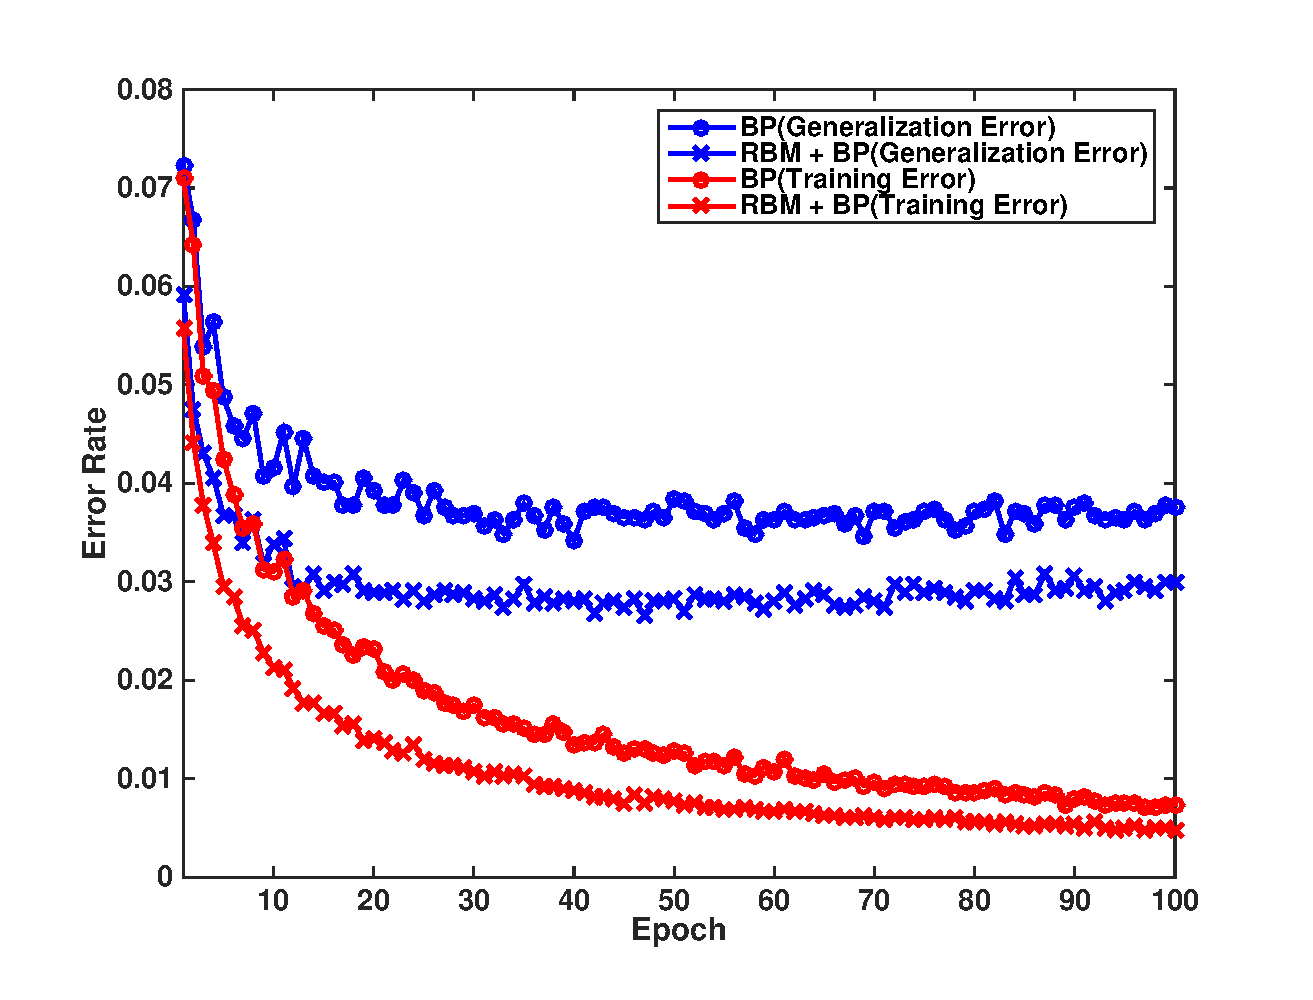
\includegraphics[width=1\linewidth]{bp_simul.eps}
\captionof{figure}{Error rates vs. epoch for BP and RBM + BP methods.}
\label{fig:bp_result}
\end{center}

\section{Conclusion}
For both methods, each update is guaranteed to lower the training error. However, it is not the case for the generalization error and we observe overfitting for both BP and RBM + BP methods, which can be seen in  Figure \ref{fig:bp_result}. In conclusion, the training method which combines the RBM and the back propagation outperforms the training method which only uses the back propagation. It is because the RBM + BP method is a generative classifier whereas the BP method is a discriminative classifier. In the RBM + BP, by training restricted Boltzmann machine which is an unsupervised learning, the joint distribution of visible and hidden nodes are learned. This provides the RBM + BP with much more information compared to the BP method about the data. This extra information causes the RBM + BP method to have both lower training and generalization errors than the BP method.  

\nocite{*} % Insert publications even if they are not cited in the poster
\small{ % Reduce the font size in this block
\bibliographystyle{unsrt}
\bibliography{sample} % Use sample.bib as the bibliography file
}

\end{document}
